% move all configuration stuff into one file so we can focus on the content
\documentclass[aspectratio=169,hyperref={pdfpagelabels=false,colorlinks=true,linkcolor=white,urlcolor=lightblue},xcolor={table},t]{beamer}

%%%%%%%%%%%%%%%%%%%%%%%%%%%%%%%%%%%%%%%%%%%%%%%%%%%%%%%%%%%%%%%%%%%%%%%%%%%%%%%%%%
%%%%%%%%%%%%%%%%%%%%%%%%%%%%%%%%%%%%%%%%%%%%%%%%%%%%%%%%%%%%%%%%%%%%%%%%%%%%%%%%%%
% packages
\usepackage{pict2e}
\usepackage{epic}
\usepackage{amsmath,amsfonts,amssymb}
\usepackage{units}
\usepackage{fancybox}
\usepackage[absolute,overlay]{textpos} 
%\usepackage[table]{xcolor}
\usepackage{animate}
\usepackage{gensymb}
%\usepackage{graphicx}
%\usepackage{longtable}
\usepackage{multirow}
\usepackage{silence}
\usepackage{tikz}
\usepackage[backend=bibtex,style=ieee]{biblatex}
\AtEveryCitekey{\iffootnote{\tiny}{}}
%\addbibresource{include/references}



% fontsize
\let\Tiny=\tiny

%%%%%%%%%%%%%%%%%%%%%%%%%%%%%%%%%%%%%%%%%%%%%%%%%%%%%%%%%%%%%%%%%%%%%%%%%%%%%%%%%%
%%%%%%%%%%%%%%%%%%%%%%%%%%%%%%%%%%%%%%%%%%%%%%%%%%%%%%%%%%%%%%%%%%%%%%%%%%%%%%%%%%
% warnings
\pdfsuppresswarningpagegroup=1
\WarningFilter{biblatex}{Patching footnotes failed}
\WarningFilter{latexfont}{Font shape}
\WarningFilter{latexfont}{Some font shapes}
\WarningFilter{gensymb}{Not defining}


%%%%%%%%%%%%%%%%%%%%%%%%%%%%%%%%%%%%%%%%%%%%%%%%%%%%%%%%%%%%%%%%%%%%%%%%%%%%%%%%%%
%%%%%%%%%%%%%%%%%%%%%%%%%%%%%%%%%%%%%%%%%%%%%%%%%%%%%%%%%%%%%%%%%%%%%%%%%%%%%%%%%%
% colors
\definecolor{gtgold}{rgb}{.914, .664, 0} %0e7eed {rgb}{0.88,0.66,1,0.06} [234, 170, 0]/256 %96caff
\definecolor{darkgray}{rgb}{.15, .15, .15}
\definecolor{lightblue}{HTML}{0e7eed}
\definecolor{highlight}{rgb}{0, 0, 1} %_less!40

%%%%%%%%%%%%%%%%%%%%%%%%%%%%%%%%%%%%%%%%%%%%%%%%%%%%%%%%%%%%%%%%%%%%%%%%%%%%%%%%%%
%%%%%%%%%%%%%%%%%%%%%%%%%%%%%%%%%%%%%%%%%%%%%%%%%%%%%%%%%%%%%%%%%%%%%%%%%%%%%%%%%%
% relative paths
\graphicspath{{../graph/}}


%%%%%%%%%%%%%%%%%%%%%%%%%%%%%%%%%%%%%%%%%%%%%%%%%%%%%%%%%%%%%%%%%%%%%%%%%%%%%%%%%%
%%%%%%%%%%%%%%%%%%%%%%%%%%%%%%%%%%%%%%%%%%%%%%%%%%%%%%%%%%%%%%%%%%%%%%%%%%%%%%%%%%
% units
\setlength{\unitlength}{1mm}

%%%%%%%%%%%%%%%%%%%%%%%%%%%%%%%%%%%%%%%%%%%%%%%%%%%%%%%%%%%%%%%%%%%%%%%%%%%%%%%%%%
%%%%%%%%%%%%%%%%%%%%%%%%%%%%%%%%%%%%%%%%%%%%%%%%%%%%%%%%%%%%%%%%%%%%%%%%%%%%%%%%%%
% math
\DeclareMathOperator*{\argmax}{argmax}
\DeclareMathOperator*{\argmin}{argmin}
\DeclareMathOperator*{\atan}{atan}
\DeclareMathOperator*{\arcsinh}{arcsinh}
\DeclareMathOperator*{\sign}{sign}
\DeclareMathOperator*{\tcdf}{tcdf}
\DeclareMathOperator*{\si}{sinc}
\DeclareMathOperator*{\princarg}{princarg}
\DeclareMathOperator*{\arccosh}{arccosh}
\DeclareMathOperator*{\hwr}{HWR}
\DeclareMathOperator*{\flip}{flip}
\DeclareMathOperator*{\sinc}{sinc}
\DeclareMathOperator*{\floor}{floor}
\newcommand{\e}{{e}}
\newcommand{\jom}{\mathrm{j}\omega}
\newcommand{\jOm}{\mathrm{j}\Omega}
\newcommand   {\mat}[1]    		{\boldsymbol{\uppercase{#1}}}		%bold
\renewcommand {\vec}[1]    		{\boldsymbol{\lowercase{#1}}}		%bold

%%%%%%%%%%%%%%%%%%%%%%%%%%%%%%%%%%%%%%%%%%%%%%%%%%%%%%%%%%%%%%%%%%%%%%%%%%%%%%%%%%
%%%%%%%%%%%%%%%%%%%%%%%%%%%%%%%%%%%%%%%%%%%%%%%%%%%%%%%%%%%%%%%%%%%%%%%%%%%%%%%%%%
% media9
\newcommand{\includeaudio}[1]{
\href{run:audio/#1.mp3}{
\includegraphics[width=5mm, height=5mm]{graph/SpeakerIcon}}}

\newcommand{\includeanimation}[4]{{\begin{center}
                        \animategraphics[autoplay,loop,scale=.7]{#4}{animation/#1-}{#2}{#3}        
                        \end{center}
                        \addreference{matlab source: \href{https://github.com/alexanderlerch/ACA-Plots/blob/master/matlab/animate#1.m}{matlab/animate#1.m}}}
                        \inserticon{video}}
                        
%%%%%%%%%%%%%%%%%%%%%%%%%%%%%%%%%%%%%%%%%%%%%%%%%%%%%%%%%%%%%%%%%%%%%%%%%%%%%%%%%%
%%%%%%%%%%%%%%%%%%%%%%%%%%%%%%%%%%%%%%%%%%%%%%%%%%%%%%%%%%%%%%%%%%%%%%%%%%%%%%%%%%
% other commands
\newcommand{\question}[1]{%\vspace{-4mm}
                          \setbeamercovered{invisible}
                          \begin{columns}[T]
                            \column{.9\textwidth}
                                \textbf{#1}
                            \column{.1\textwidth}
                                \vspace{-8mm}
                                \begin{flushright}
                                     
\includegraphics[width=.9\columnwidth]{graph/question_mark}
                                \end{flushright}
                                \vspace{6mm}
                          \end{columns}\pause\vspace{-12mm}}

\newcommand{\toremember}[1]{
                        \inserticon{lightbulb}
                        }

\newcommand{\matlabexercise}[1]{%\vspace{-4mm}
                          \setbeamercovered{invisible}
                          \begin{columns}[T]
                            \column{.8\textwidth}
                                \textbf{matlab exercise}: #1
                            \column{.2\textwidth}
                                \begin{flushright}
                                     \includegraphics[scale=.5]{graph/logo_matlab}
                                \end{flushright}
                                %\vspace{6mm}
                          \end{columns}}

\newcommand{\addreference}[1]{  
                  
                    \begin{textblock*}{\baselineskip }(.98\paperwidth,.5\textheight) %(1.15\textwidth,.4\textheight)
                         \begin{minipage}[b][.5\paperheight][b]{1cm}%
                            \vfill%
                             \rotatebox{90}{\tiny {#1}}
                        \end{minipage}
                   \end{textblock*}
                    }
                    
\newcommand{\figwithmatlab}[1]{
                    \begin{figure}
                        \centering
                        \includegraphics[scale=.7]{#1}
                        %\label{fig:#1}
                    \end{figure}
                    
                    \addreference{matlab source: \href{https://github.com/alexanderlerch/MUSI-6202/blob/main/matlab/plot#1.m}{plot#1.m}}}
\newcommand{\figwithref}[2]{
                    \begin{figure}
                        \centering
                        \includegraphics[scale=.7]{#1}
                        \label{fig:#1}
                    \end{figure}
                    
                    \addreference{#2}}  
                                    
\newcommand{\inserticon}[1]{
                    \begin{textblock*}{100mm}(14.5cm,7.5cm)
                        \includegraphics[height=.8cm,keepaspectratio]{graph/#1}
                    \end{textblock*}}            

%%%%%%%%%%%%%%%%%%%%%%%%%%%%%%%%%%%%%%%%%%%%%%%%%%%%%%%%%%%%%%%%%%%%%%%%%%%%%%%%%%
%%%%%%%%%%%%%%%%%%%%%%%%%%%%%%%%%%%%%%%%%%%%%%%%%%%%%%%%%%%%%%%%%%%%%%%%%%%%%%%%%%
% counters
\newcounter{i}
\newcounter{j}
\newcounter{iXOffset}
\newcounter{iYOffset}
\newcounter{iXBlockSize}
\newcounter{iYBlockSize}
\newcounter{iYBlockSizeDiv2}
\newcounter{iXBlockSizeDiv2}
\newcounter{iDistance}

\newcommand{\IEEELink}{https://ieeexplore.ieee.org/servlet/opac?bknumber=9965970}



\subtitle{Part 12: Non-linear Quantization}

%%%%%%%%%%%%%%%%%%%%%%%%%%%%%%%%%%%%%%%%%%%%%%%%%%%%%%%%%%%%%%%%%%%%%%%%%%%%
\begin{document}
    % generate title page
	\title[]{Digital Signal Processing for Music}   
\author[alexander lerch]{alexander lerch} 
%\institute{~}
%\date[Alexander Lerch]{}
\titlegraphic{\vspace{-16mm}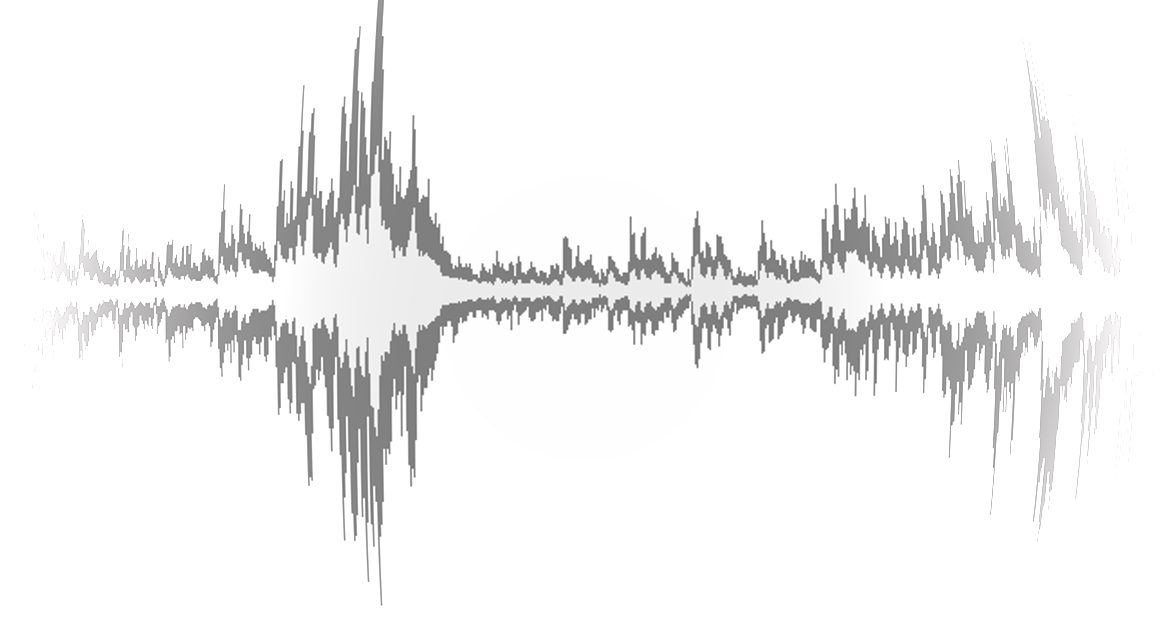
\includegraphics[width=\textwidth,height=3cm]{title}}


\begin{frame}
    \titlepage
    %\vspace{-5mm}
    \begin{flushright}
        \href{http://www.gtcmt.gatech.edu}{
\includegraphics[height=.8cm,keepaspectratio]{../shared/Logo_GTCMT_black}}
    \end{flushright}
\end{frame}


\section[intro]{introduction}

\begin{frame}{non-linear quantization}{introduction: linear quantization---SNR \& PDF}
		\begin{equation*}
			SNR = 6.02\cdot w + c_{\mathrm{S}}\quad [dB]
		\end{equation*}
		\pause
        \bigskip
		$\Rightarrow c_{\mathrm{S}}$ depends on signal's PDF (and scaling)
		\begin{table}
			\centering
			\begin{footnotesize}
				\begin{tabular}{clc}
				\hline
				\textbf{PDF} & \textbf{SNR}\\
				\hline
				square wave & $c_S =  4.8$\\
				sine wave & $c_S =  1.8$\\
				rect & $c_S =  0$\\
				tri & $c_S \approx  -3$\\
				Gauss & $c_S \approx  -7$\\
				Laplace & $c_S \approx  -9$\\
				speech & $c_S \approx  -10\ldots -15$\\
				\hline
				\end{tabular}
			\end{footnotesize}
		\end{table}
	\end{frame}	
    
	\begin{frame}{non-linear quantization}{introduction}
		\textbf{idea}: quantize frequent signal values at higher resolution
		
		\begin{itemize}
			\item<2-> \textbf{approach 1 }	
				\begin{enumerate}
					\item	flatten PDF (companding)
					\item	linear quantization
					\item	extract signal (expanding)
				\end{enumerate}
			\only<2>{
            \begin{figure}
                \begin{center}
                    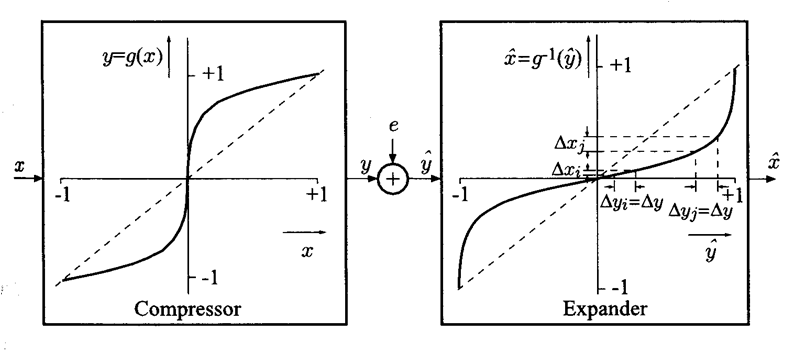
\includegraphics[scale=0.5]{Graph/quant_compexp}
                \end{center}
            \end{figure}
            }
			\only<3->{
            \begin{figure}
                \begin{center}
                    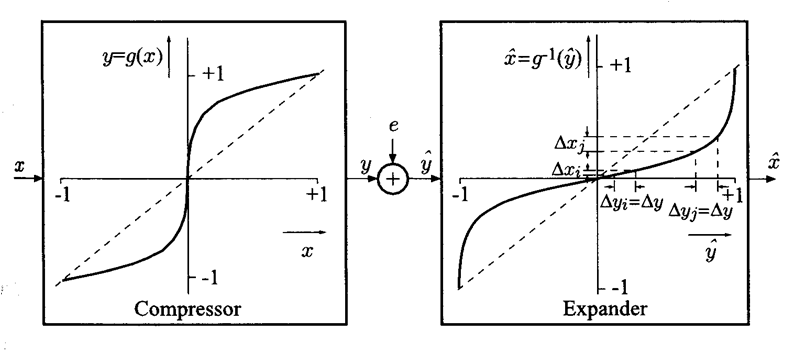
\includegraphics[scale=0.2]{Graph/quant_compexp}
                \end{center}
            \end{figure}
            }
            \item<3-> \textbf{approach 2 }	
				\begin{enumerate}
					\item	adapt quantization step size to PDF
				\end{enumerate}
            \bigskip
            \item<4->[$\Rightarrow$] both approaches are equivalent in their result
		\end{itemize}
	\end{frame}	

\section[A-law]{A-Law quantization}
	\begin{frame}{non-linear quantization}{A-Law quantization  (ITU-T G.711) 1/3}
		\begin{equation*}
			F(x)	= sign(x)\left\lbrace
					\begin{array}{ll} 
			          \frac{A|x|}{1+\log(A)}, & |x| \leq \frac{1}{A}\\ 
			          \frac{1+\log(A|x|)}{1+\log(A)}, & \frac{1}{A} \leq |x| \leq 1\\ 
          			\end{array} 
          			\right.
		\end{equation*}
        \bigskip
		\begin{equation*}
			F^{-1}(y)	= sign(y)\left\lbrace
					\begin{array}{ll} 
			          \frac{|y|(1+\log(A))}{A}, & |y| \leq \frac{1}{1+\log(A)}\\ 
			          \frac{\exp\big(|y|(1+\log(A))-1\big)}{A}, & \frac{1}{1+\log(A)} \leq |y| \leq 1\\ 
          			\end{array} 
          			\right.
		\end{equation*}
		\bigskip
		\bigskip
        with $A = 87.7$
        
        \pause
        \begin{itemize}
            \item   linear and high resolution for small amplitudes
            \item   log and increasingly low resolution for high amplitudes
        \end{itemize}
	\end{frame}	

	\begin{frame}{non-linear quantization}{A-Law quantization 2/3}
        \vspace{-4mm}
	    \begin{figure}
			\centering
				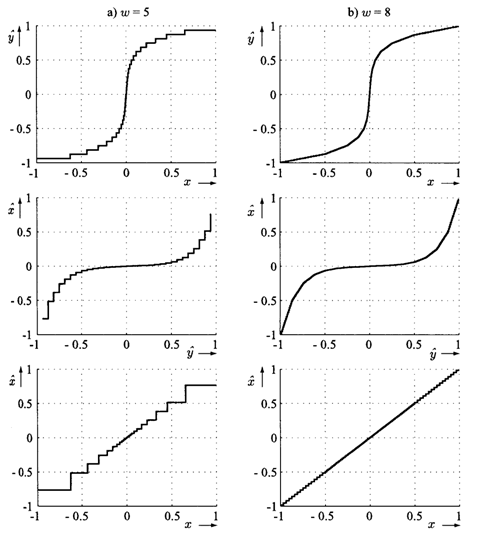
\includegraphics[scale=0.5]{Graph/a-law}
		\end{figure}
	\end{frame}

	\begin{frame}{non-linear quantization}{A-Law quantization 3/3}
	    \vspace{-5mm}
        \begin{figure}
			\centering
				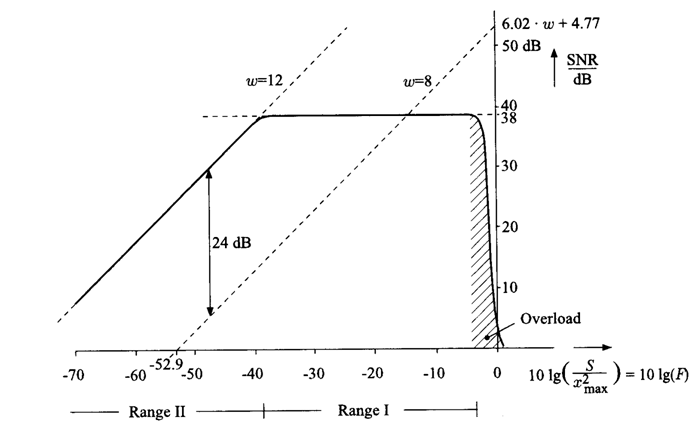
\includegraphics[scale=0.5]{Graph/snr_a-law}
		\end{figure}
        \begin{itemize}
            \item   range I: SNR is linear regardless of input level
            \item   range II: SNR increases with input level
        \end{itemize}
	\end{frame}

\section[$\mu$-law]{$\mu$-Law quantization}
	\begin{frame}{non-linear quantization}{$\mu$-Law quantization  (ITU-T G.711)}
		\begin{equation*}
			F(x)	= sign(x)\frac{\log(1+\mu|x|)}{\log(1+\mu)}
		\end{equation*}
        \bigskip
		\begin{equation*}
			F^{-1}(y)	= sign(y)\frac{1}{\mu}\left((1+\mu)^{|y|}-1\right)
		\end{equation*}
		\bigskip
		\bigskip
        with $\mu = 255$
        
        \pause
        compared to A-Law:
        \begin{itemize}
            \item   higher dynamic range
            \item   higher error at small amplitudes
        \end{itemize}
	\end{frame}	

	\section{summary}	
		\begin{frame}{non-linear quantization}{summary}
            \begin{itemize}
                \item \textbf{advantages} of non-linear quantization
                    \begin{itemize}
                        \item   takes advantage of non-uniform distribution of input
                        \item   in line with non-linear loudness perception of the ear
                        \item[$\Rightarrow$]    similar perceptual quality as higher resolution linear quantization
                    \end{itemize}
                \bigskip
                \item    \textbf{disadvantages}
                    \begin{itemize}
                        \item   processing not easily implemented in non-linear amplitude space
                        \item[$\Rightarrow$] only used for transmission   
                    \end{itemize}
            \end{itemize}
		\end{frame}
 

\end{document}

